\documentclass[11pt]{article}
\usepackage{fullpage}
\usepackage{amsmath}
\usepackage{esint}
\usepackage{cancel}
\usepackage{graphicx}
\linespread{1.1}
\usepackage{commath}
\usepackage[sc,osf]{mathpazo}
\newcommand{\Lagr}{\mathcal{L}}


\begin{document}

\title{MIE375  \\ Financial Engineering}
\author{Michael Boyadjian}
\maketitle
\pagebreak

\tableofcontents

\pagebreak

\bigskip
\bigskip
\bigskip

\section{Theory of Interest}

\subsection{Principle and Interest}
\begin{itemize}
\item \textbf{Principle:} amount invested
\item\textbf{Interest: }"rent" paid on an investment
\item Amount received after one period is $A(1+r)$
\item Two compounding rules: (i) simple (ii) compound
\end{itemize}

\subsubsection{Simple Interest}
\begin{itemize}
\item Interest is proportional to the time invested
\item At time $n$ the value is $A(1+rn)$; money grows linearly
\item Not often used in practice
$$ V = A(1+rn)$$
\begin{center}
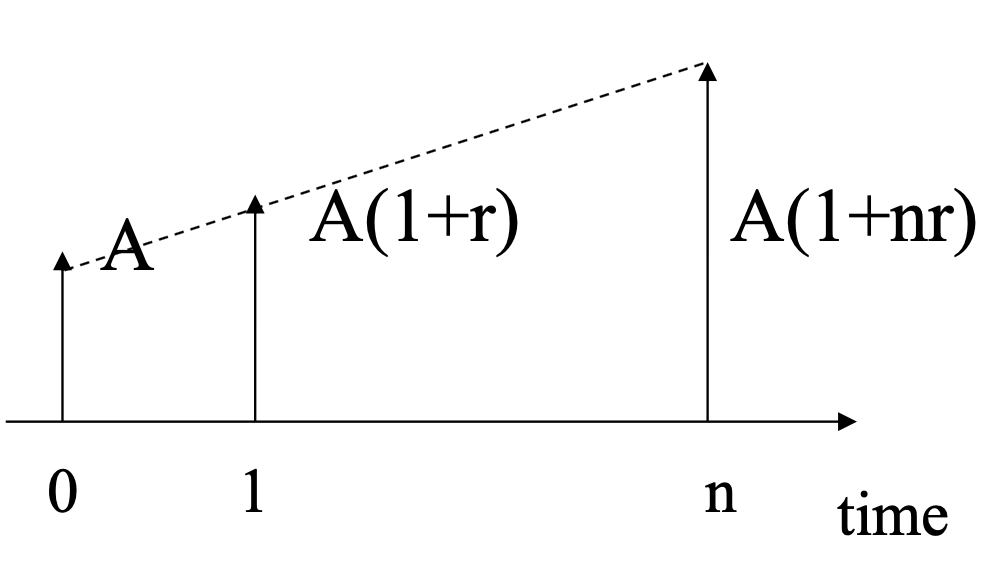
\includegraphics[scale=0.4]{simple.png} 
\end{center}
\end{itemize}

\subsubsection{Compound Interest}
\begin{itemize}
\item Interest on interest
\item At time $n$ the value is $A(1+r)^n$; money grows geometrically
$$ V = A(1+r)^n$$
\begin{center}
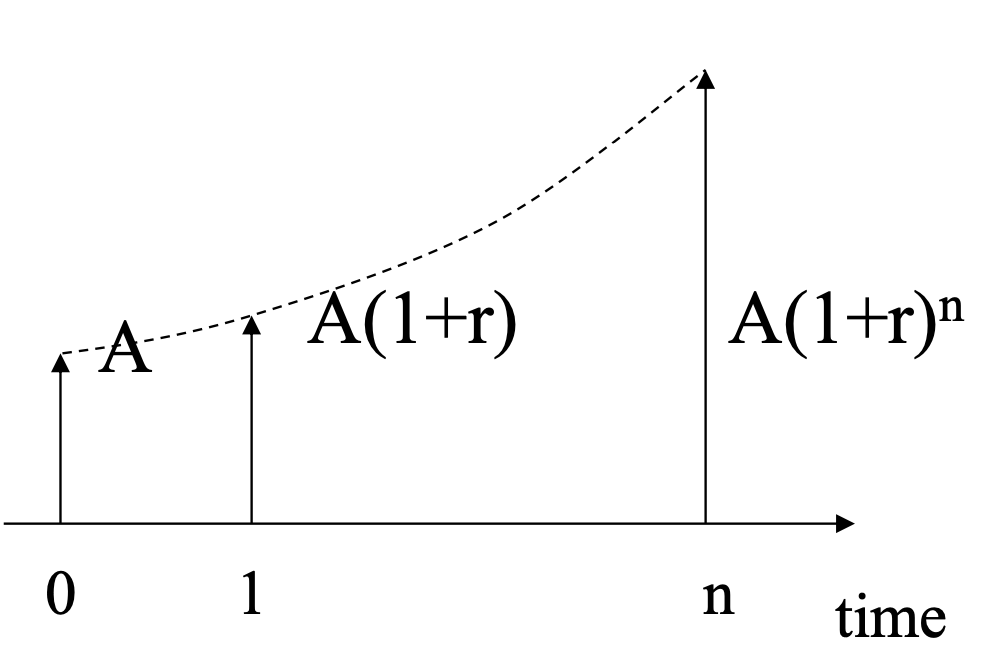
\includegraphics[scale=0.4]{compound.png} 
\end{center}
\item \textbf{Rule of 72:} Money invested at $r \%$ a year doubles in approximately $72/r$ years
\item \textbf{Nominal Interest:} At $r\%$ compounded $m$ periods per year for $k$ periods would cause money to grow by the factor $(1+ \frac{r}{m})^k$
\begin{center}
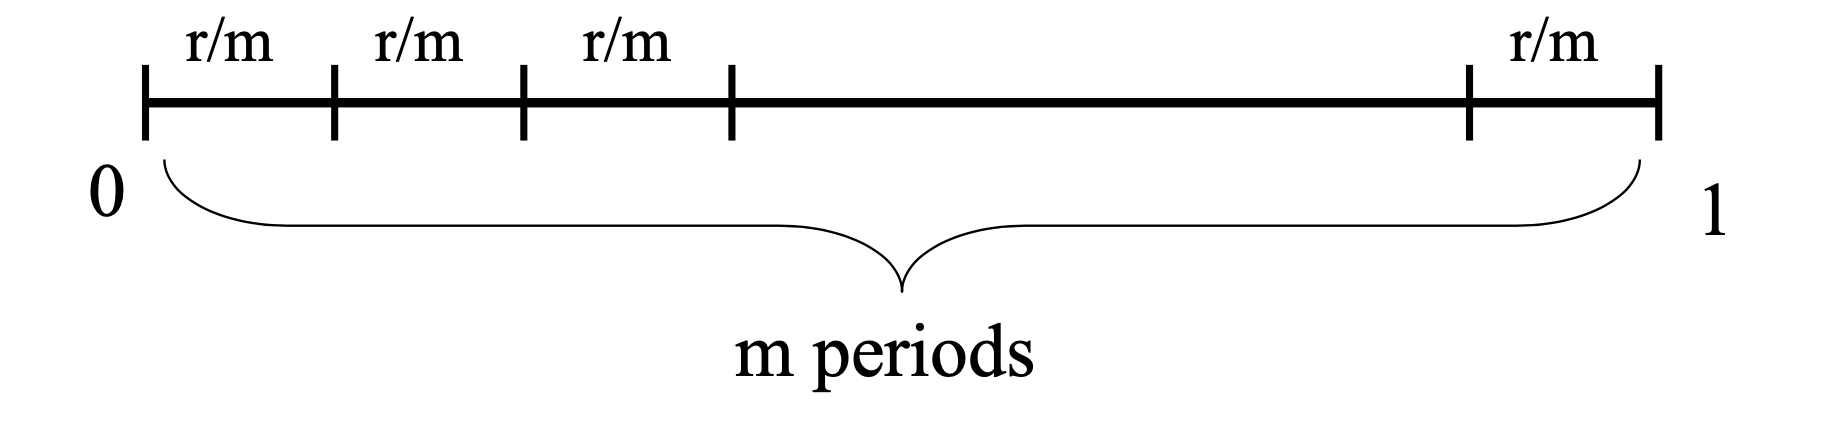
\includegraphics[scale=0.3]{nominal.png} 
\end{center}
\item \textbf{Continuous Compounding:} Take the limit of $m$ periods as $m$ approached infinity:
$$V =  \lim_{m \rightarrow \infty} \left(1 +\frac{r}{m} \right)^m = e^{rt}$$
\end{itemize}

\subsubsection{Effective Interest Rate}
\begin{itemize}
\item Interest rates usually quotes as nominal rates
\item Amount paid depends on compounding periods
\item When we compute equivalent rate with a single compounding period over the time interval of interest, we refer to this as the effective rate:
$$ r_{eff} = \left( 1 + \frac{r_{nom}}{m} \right) ^ m -1 $$
\end{itemize}

\subsubsection{Commonly Referred to Rates}
\begin{itemize}
\item \textbf{Annual Percentage Rate (APR):} Nominal annual rate of interest including all fees and charges
\item \textbf{Annual Percentage Yield (APY):} Effective annual rate of interest including all fees and charges
\item \textbf{Discount Rate:} Rate at which member banks may borrow short term funds directly from federal reserve bank 
\item \textbf{Federal Funds Rate:} Rate that banks charge each other for use of federal funds
\item \textbf{Prime Rate:} Rate that commercial banks charge their most creditworthy borrowers
\item \textbf{London Interbank Offer Rate (LIBOR):} The interest rate banks charge each other for loans (usually euros)
\end{itemize}
\pagebreak

\subsection{Present Value and Internal Rate of Return}
\subsubsection{Ideal Bank}
\begin{itemize}
\item Applies the same rate of interest to deposits and loans and has no transaction costs 
\item Two main operations:
\begin{itemize}
\item \textbf{Compounding -} Every time a cash flow is moved \textit{forward} one period, it is \textit{multiplied} by $(1+r)$
\begin{center}
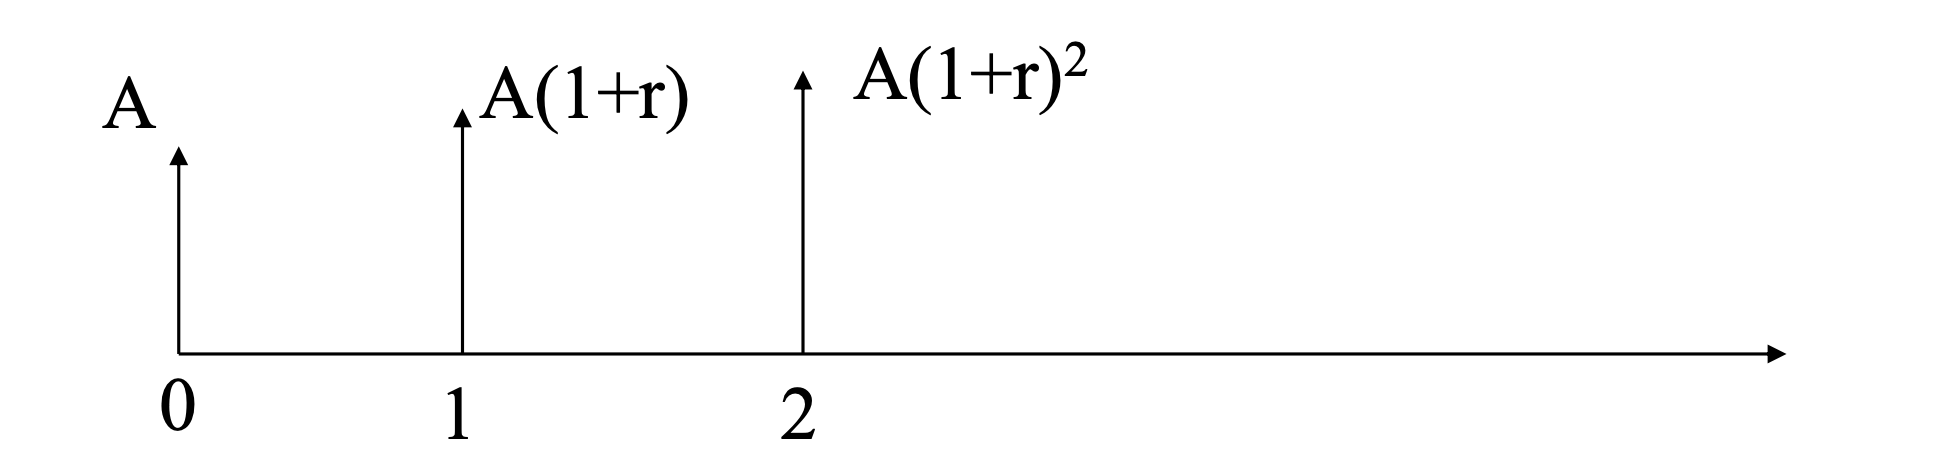
\includegraphics[scale=0.3]{compounding.png} 
\end{center}
\item \textbf{Discounting -} Every time a cash flow is moved \textit{backward} one period, it is \textit{divided} by $(1+r)$
\begin{center}
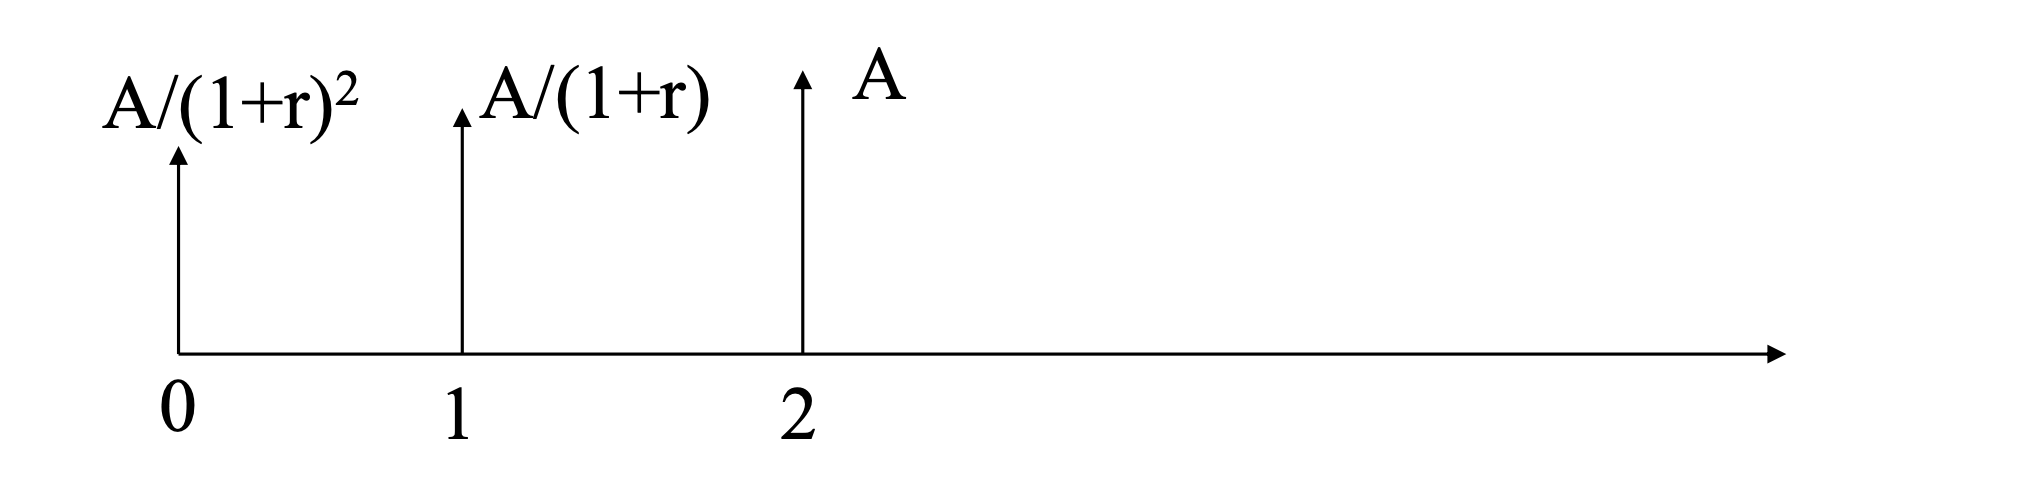
\includegraphics[scale=0.3]{discounting.png} 
\end{center}
\end{itemize}
\end{itemize}

\subsubsection{Present / Future Value}
\begin{itemize}
\item \textbf{Present Value:} Cash flows moved to present time 
$$ PV = \sum_{k=0}^{n} \frac{x_k}{(1+r)^k}$$
\item \textbf{Future Value:} Cash flows moved forward in time to the time of the final cash flow
$$ FV = PV (1+r)^n$$
\item Two cash flow streams are equivalent for an ideal bank if and only if they have the same present value 
\end{itemize}

\subsubsection{Internal Rate of Return}
\begin{itemize}
\item The return on your investment which would have the present value equal to 0
\item Let $x = (x_0, x_1, x_2, \cdots x_n)$ be a cash flow stream, the IRR of this stream is a number $r$ satisfying $PV(x) = 0$ 
$$ x_0 + \frac{x_1}{(1+r)} + \frac{x_3}{(1+r)^2} + \cdots + \frac{x_n}{(1+r)^n} = 0$$
\end{itemize}

\pagebreak

\section{Fixed Income Securities}
\subsection{Terminology}
\begin{itemize}
\item \textbf{Financial Instrument:} A legal obligation or claim having a monetary structure \textit{(e.g. stocks, bonds, mortgages, futures, insurance, etc.)}
\item \textbf{Security:} A tradable financial instrument satisfying legal and regulatory requirements 
\item \textbf{Fixed Income Security:} Securities that promise a fixed income to the holder over some span of time (\textit{e.g. bonds, mortgages, etc.)}
\end{itemize}
\subsection{Annuities}
A contract that pays the holder money periodically according to a fixed income 
\begin{itemize}
\item \textbf{Perpetuity:} Pays a fixed sum periodically forever
$$ PV = \sum_{k=1}^{\infty} \frac{A}{(1+r)^k} = \frac{A}{r} $$ 
\item \textbf{Finite Life Streams:}  Pays an annuity $A$ for $n$ periods
$$ PV = \sum_{k=1}^{\infty} \frac{A}{(1+r)^k} = \frac{A}{r} \left( 1 - \frac{1}{(1+r)^n} \right)$$ 
Alternatively, if solving for the value of the annuity :
$$ A = \frac{r P}{ \left( 1 - \frac{1}{(1+r)^n} \right) } $$ 
\end{itemize}
\subsection{Bonds}
An agreement to pay money according to the rules of the issue
\begin{itemize}
\item \textbf{Face Value / Par Value / Principle:} An amount to be paid at the maturity date 
\item \textbf{Coupon Payments:} Amount paid periodically expressed as a percentage of face value, last paid at maturity 
\item \textbf{Zero-Coupon Bond:} No coupons are paid out, only payoff is face value at maturity
\item Bond price quotes ignore accrued interest, which must be added to the price; must pay the previous owner their portion of the next coupon payment
\item Market bond prices are referred to as the \textit{clean} price. When accrued interest is included, then it is referred to as the \textit{dirty} or \textit{cash} price.
\end{itemize}

\subsubsection{Price and Yield}
The internal rate of return of a bond cash flow stream is referred to as the yield ($\lambda$). The yield captures the “rate of return” that one would obtain by purchasing the bond and holding it to maturity. 
\begin{center}
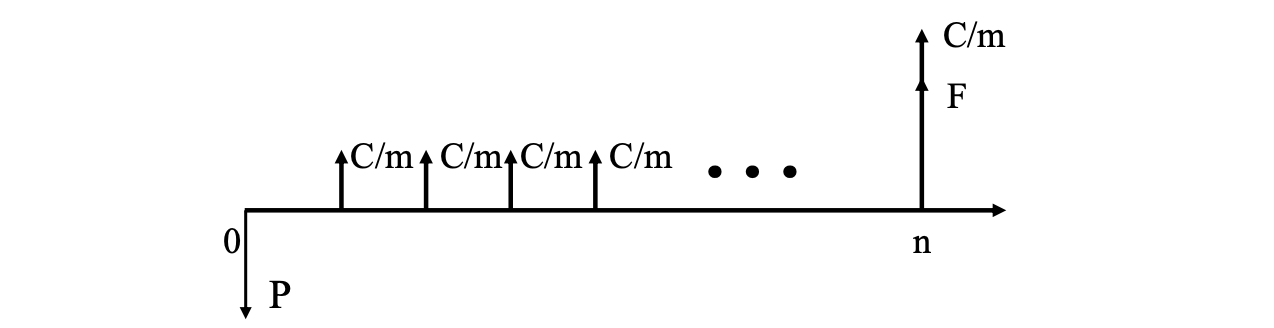
\includegraphics[scale=0.6]{yield.png} 
\end{center}
We use the following formula to relate the price and yield with $n$ remaining coupon payments:
$$ P = \frac{F}{\left(1+\frac{\lambda}{m}\right)^n} + \frac{C/m}{\lambda / m } \left(1 - \frac{1}{\left(1+\frac{\lambda}{m}\right)^n}\right) $$
The longer the time to maturity, the more sensitive the price of the bond is to the yield.  We can see this in the Price-Yield curve:
\begin{center}
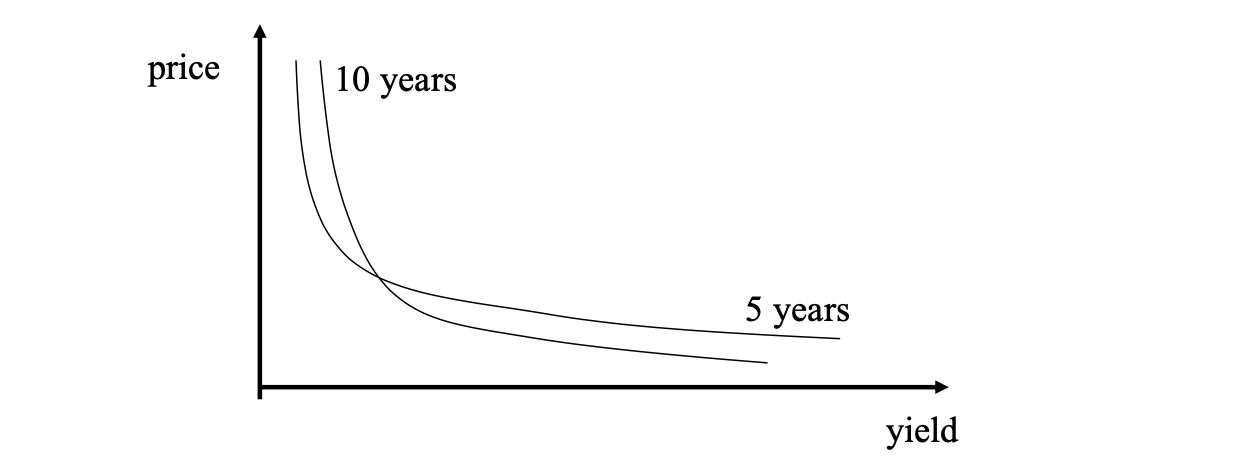
\includegraphics[scale=0.7]{py.png} 
\end{center}
\subsubsection{Duration}
The maturity time of a bond is related to the sensitivity of the bond price to the yield. With coupons, the maturity time does not exactly correspond to the sensitivity.  \\ \\ We define the \textbf{Macaulay Duration}, which is a weighted average of times to cash flows: \\ \smallskip
$$ D = \frac{PV(t_1)t_1 + PV(t_2)t_2 + \cdots + PV(t_n)t_n  }{PV_{TOTAL}} $$ 
\\
This is a weighted average of times, quoted in years.  For a coupon bond, $macaulay \; duration < maturity \; date$, while for a zero-coupon bond $macaulay \; duration = maturity \; date$.  \\ \\
The Macaulay Duration for a bond with coupon rate per year, $C$, yield, $\lambda$,  periods per year, $m$, and periods remaining, $n$, is given by:
$$D = \frac{1+ \frac{\lambda}{m}}{ \lambda} - \frac{1+\frac{\lambda}{m} + n (\frac{C}{m} - \frac{\lambda}{m}
)}{C[(1+\frac{\lambda}{m})^n -1] + \lambda} $$ 
We then define the \textbf{Modified Duration} to calculate the sensitivity of a bond to yield exactly. $$D_m = - \frac{1}{P(\lambda_0} \left. \frac{dP(\lambda)}{d\lambda} \right|_{\lambda=\lambda_0} \approx - \frac{1}{P} \frac{\Delta P}{\Delta \lambda}$$ 
The Macaulay Duration and Modified Duration are then related through the following equation: 
$$ D_m = \frac{D}{1+\frac{\lambda}{m}}$$
In the case of continuous compounding, $D_m = D$. \\ \\
Finally, if composing a portfolio of bonds, given fixed income securities with prices $P_i$,  durations, $D_i$,  and weights,  $w_i = P_i / P$,  $i = 1,2, \cdots m$, the aggregate portfolio of all of these has price $P$ and duration $D$ given by
$$ P = P_1 + P_2 + \cdots + P_m$$ 
$$ D = D_1w_1 +D_2 w_2+ \cdots + D_mw_m$$ 

\pagebreak

\section{Term Structure of Interest Rates}

\subsection{Yield Curve}
In general, yields on bonds of different maturities are different.  If we plot $yield$ vs $time$ to maturity for bonds, we call the resulting curve the yield curve. The yield curve is not exactly what we want since there may be coupons, etc. We would really like to know the interest rate on a cash flow at time $t$, with no intermediate cash flows.
\begin{center}
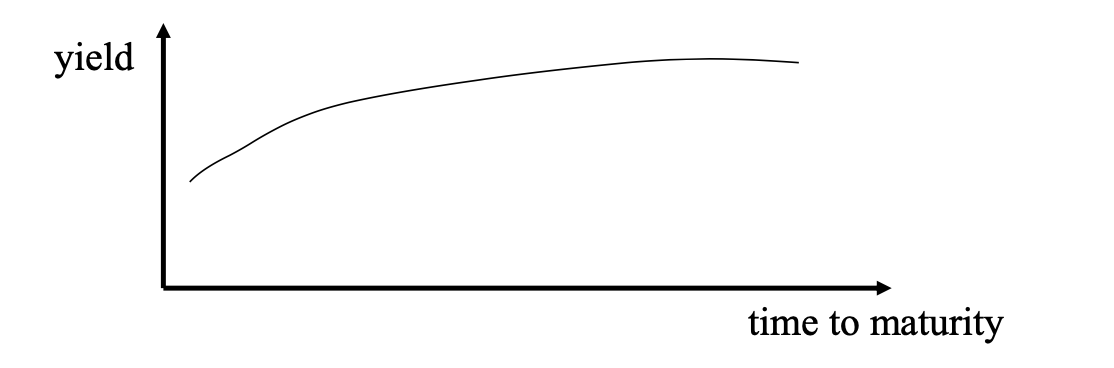
\includegraphics[scale=0.6]{yieldcurve.png} 
\end{center}
\subsection{Spot Rates}
Interest rates for a specific time period are called spot rates. They can be quted as being compounded (i) yearly, (ii) $m$ periods / year, or (iii) continuously.  When computing $PV$ the spot rate corresponding to the time of the cash flow must be used. If we know the price of a zero coupon bond, it's yield will be the spot rate:
$$ P = Fe^{-st}$$
There are 3 equations we can use from a portfolio of bonds to determine the spot rate. 
\begin{align*}
xP_1 + yP_2 &= P_0 \\ 
xC_1 +yC_2 &= C_0 \\ 
xF_1 + yF_2 &= F_0 
\end{align*}
We solve the system of equations to determine $x$  and $y$ and from there we can find the price and spot rate.
\subsection{Forward Rates}
Interest rates for money to be borrowed between two dates in the future, but under terms agreed upon today. $f_{t_1, t_2}$ represents the forward rate between $t_1$ and $t_2$ 
$$ (1+ s_i)^i (1 +f_{i,j})^{j-1} = (1+s_j)^j$$
When we consider rates that only span one period, we refer to those as spot rates 
\subsection{Expectation Dynamics}
We don't know what actual future rates will be when the future time arrives. Using forward rates to predict is called expectation dynamics.  According to the \textbf{Invariance Theorem}, if interest rates evolve according to expectation dynamics then money invested invested for $n$ years will grow by $(1+s_n)^n$ regardless of strategy.
\begin{center}
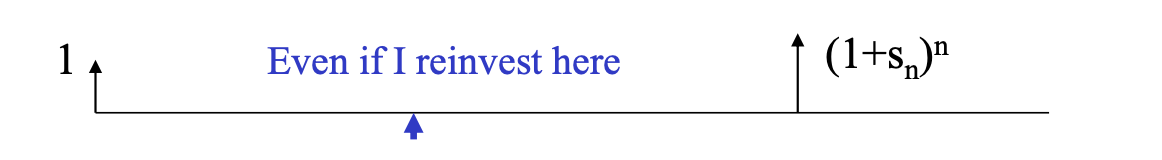
\includegraphics[scale=0.6]{invariance.png} 
\end{center}
\subsection{Immunization}
We construct a portfolio of bonds which is protected against changes in interest rates.  The portfolio is constructed with present value $P$ and duration $D$ equal to those of your obligation. 
\begin{align*}
xP_1 + yP_2 &= P \\
x \frac{P_1}{P} D_1 + y \frac{P_2}{P} D_2 &= D 
\end{align*}
Solving for $x$ and $y$ we can determine our portfolio. The idea behind this immunization is Taylor expansion
$$ P(\lambda) = P(\lambda_0) + P'(\lambda_0) (\lambda - \lambda_0) + \frac{1}{2} P'' (\lambda_0) (\lambda - \lambda_0)^2 + \cdots $$
\pagebreak

\section{Applied Interest Rate Analysis}

\subsection{Dynamic Programming}
Running present value is a recursive method for calculating present value.  This satisfies the recursive formula: \\  $$ PV(k) = x_k + \frac{PV(k+1)}{1+f_{k,k+1}}$$ \\
Dynamic decisions are problems where cash flows depend on decisions that will be made at future times. These problems are often similar to running present value calculations, except we have a decision to make at each time.  See the fishing problem for an example of how this is used.  Remember to "solve the problem backwards"!

\subsection{Capital Budgeting}
\begin{itemize}
\item Deciding on which projects to invest in 
\item Need to choose a portfolio which maximizes the net present value
\item Either select entire project or not at all
\item Optimal capital budgeting: 
\begin{itemize}
\item $ \max \sum_{i=1}^n b_ix_i $ (present value)
\item $ \max \sum_{i=1}^n c_ix_i < c$ (budget constraint)
\item $x_i = 0$ or $x_i = 1$ (all or nothing)
\end{itemize}
\end{itemize}
\pagebreak

\section{Mean-Variance Portfolio Theory}
\subsection{Probability}
Review of some important probability concepts that are used in portfolio theory
\begin{itemize}
\item \textbf{Expectation / Mean}
$$ \bar{x} = E[x] = \sum_{i=0}^n x_ip_i $$
\item \textbf{Variance}
$$ VAR[X] = E[X^2] - (E[X])^2$$ 
$$ VAR[aX \pm bY] = a^2VAR[X] + b^2VAR[Y]$$
$$ \sigma_x = \sqrt{VAR[X]}$$
\item \textbf{Covariance}
$$ COV(X_1, X_2) = E[X_1X_2] - \bar{x}_1\bar{x}_2 = \sigma_{12}$$
$$ COV(X_1, X_2) = 0  \text{ if } x_1 \text{ and } x_2 \text { are independent}$$
$$ COV(X_1, X_1) = VAR[X_1]$$
$$ COV(aX + bY + f, cX+dY+e) = acVAR[X] +(ad-bc) COV[X,Y] + bdVAR[Y]$$
\item \textbf{Correlation}
$$ \rho_{12} = \frac{\sigma_{12}}{\sigma_1 \sigma_2}$$
\end{itemize}

\subsection{Portfolio Returns}
Assume there is an asset whose current value is $X_0$ and its value one year later is $X_1$. It's rate of  return and total return are expressed as:
$$ r = \frac{X_1-X_0}{X_0} \quad \quad R = \frac{X_1}{X_0}$$
Now, assuming we had a portfolio of $n$  assets, we can describe this through the following table: \\ 
\begin{center}
\begin{tabular}{c|c|c|c} 
\textbf{Asset} & $\$$ \textbf{Invested} & \textbf{Weights} & \textbf{Return} \\
\hline \hline
1    &    $X_0^1$        &      $w_1 = \frac{X_0^1}{X_0 } $      & $r_1$  \\
2    &   $X_0^2$        &      $w_2 = \frac{X_0^2}{X_0 } $      & $r_2$  \\
$\cdots$ & $\cdots$ & $\cdots$ & $\cdots$ \\
n   &    $X_0^n$        &      $w_n = \frac{X_0^n}{X_0 } $      & $r_n$  \\
\hline 
\textit{TOTAL}  & $X_0 = \sum_{i=1}^n X_0^i$ & $\sum_{i=1}^n w_i = 1$  & $r_p = \sum_{i=1}^n w_ir_i$  \\
\end{tabular}
\end{center}
\pagebreak
As seen in the table above, the return of the portfolio is given by:
$$ r_p = \sum_{i=1}^n w_ir_i $$ 
\begin{itemize}
\item The returns, $r_i$, on the individual assets are random
\item $r_p$ is a weighted sum of the random variables $r_i$
\item To determine the expected return of a portfolio, or the variance / standard deviation of the return, must start with this
\end{itemize}
The expected return of a portfolio is then given by :
$$\bar{ r}_p = E[r_p] =  \sum_{i=1}^n w_i\bar{r}_i $$ 
The variance of the return of a portfolio is given by: 
$$ \sigma_p^2 = VAR[r_p] = \sum_{i=1}^{n}\sum_{j=1}^n w_i w_j \sigma_{ij} $$
When the assets are uncorrelated, this becomes:
$$ \sigma_p^2 = VAR[r_p] = \sum_{i=1}^{n} w_i^2\sigma_{i}^2 $$

\subsection{Short Selling}
Short selling corresponds to borrowing an asset and selling it with the understanding that you'll buy it back at some point in the future. In portfolio terms, the asset is given a negative weight $w_i$. Money is made if the price drops.

\subsection{Portfolio Diagrams}
\begin{center}
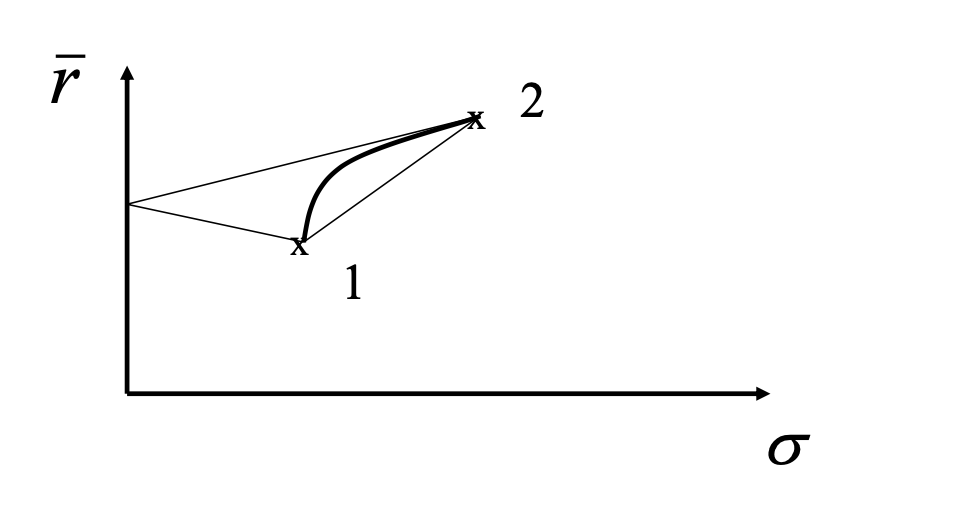
\includegraphics[scale=0.6]{port.png} 
\end{center}

\subsection{Minimum-Variance Set}
For a given mean return, you would like to minimize your risk or variance
\begin{center}
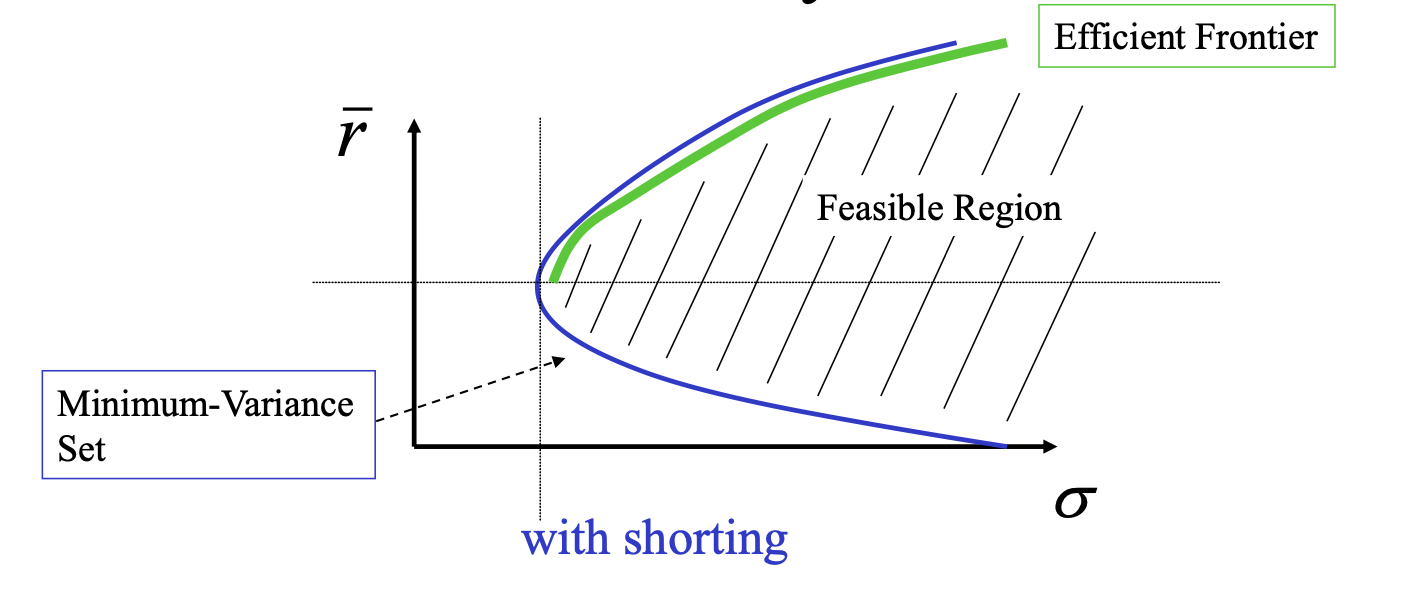
\includegraphics[scale=0.6]{minvar.png} 
\end{center}
If you're risk averse. then:
\begin{itemize}
\item for a given mean return, you will minimize the variances or "risk"
\item always want your portfolio to be on the minimum variance set
\item for a given variance, you will maximize your mean return
\item hence, you will want to be on the top portion of the minimum variance set, known as the efficient frontier
\end{itemize}

\subsection{Markowitz Theory}
Markowitz formulated the problem of being on the efficient frontier as an optimization problem. Assuming there are $n$ risky assets with mean returns $\bar{r}_i, \bar{r}_2, \cdots, r_n$ and covariances $\sigma_{ij}$ for $i,j = 1 \cdots n$, we want to minimize (1) subject to (2) and (3). Note that  we allow short selling and we assume all assets are risky.
\begin{equation}
 \frac{1}{2} \sum_{i=1}^n \sum_{j=1}^n w_iw_j \sigma_{ij} = \frac{1}{2}
\end{equation}
\begin{equation}
 \sum_{i=1}^n w_i\bar{r}_i = \bar{r}_p 
\end{equation}
\begin{equation}
 \sum_{i=1}^n w_i =1 
\end{equation}
\pagebreak
\subsubsection{Solving a General Optimization}
Given the following optimization problem:
$$ \min f(x,u)$$
$$ \text{subject to } g_1(x,u) = c_1 \quad \text{and} \quad g_2(x,u) = c_2 $$ 
We go through the following steps to solve this:
\begin{enumerate}
\item Convert all constraints to 0 on the RHS
$$ g_1(x,u) - c_1  = 0$$
$$ g_2(x,u) - c_2 = 0$$
\item Associate a Lagrange multiplier with each constraint
$$ g_1(x,u) - c_1  = 0 \rightarrow \lambda_1$$
$$ g_2(x,u) - c_2 = 0 \rightarrow \lambda_2$$
\item Form a Lagrangian by subtracting from the objective each constraint multiplied by its Lagrange multiplier
$$ \Lagr(x, u,\lambda_1, \lambda_2) = f(x,u) - \lambda_1(g_1(x,u) - c_1) - \lambda_2(g_2(x,u) - c_2)$$
\item Compute the partial derivatives and set them to 0
$$ \frac{\partial \Lagr}{\partial x} = \frac{\partial f}{\partial x } - \lambda_1 \frac{\partial g_1}{\partial _x} - \lambda_2 \frac{\partial g_2}{\partial _x} = 0$$
$$ \frac{\partial \Lagr}{\partial u} = \frac{\partial f}{\partial u } - \lambda_1 \frac{\partial g_1}{\partial _u} - \lambda_2 \frac{\partial g_2}{\partial _u} = 0$$
$$ -\frac{\partial \Lagr}{\partial \lambda_1} = g_1(x,u) - c_1$$
$$ -\frac{\partial \Lagr}{\partial \lambda_2} = g_2(x,u) - c_2$$
\item Solve the equations for $x, u, \lambda$ to find the optimal solution
\end{enumerate}
\subsubsection{Two-Fund Theorem}
Assuming (i) short selling is allowed, (ii) all assets are risky, and (iii) all investors have the same estimates of mean, variance, and covariance, investors seeking minimum variance portfolios need only invest in linear combinations of two minimum variance funds. Only two efficient funds need to exists and everyone else can invest in them!

\subsubsection{Inclusion of a Risk Free Asset}
Now assume there is a risk free asset with return $r_f$.  We want to combine the risk free asset with the risky portfolio.  This results in the following:
\begin{align*}
mean &= \alpha r_f + (1-\alpha) \bar{r} \\
variance &= (1-\alpha)^2 \sigma^2 \\
standard \; deviation & = (1-\alpha) \sigma
\end{align*}
\begin{center}
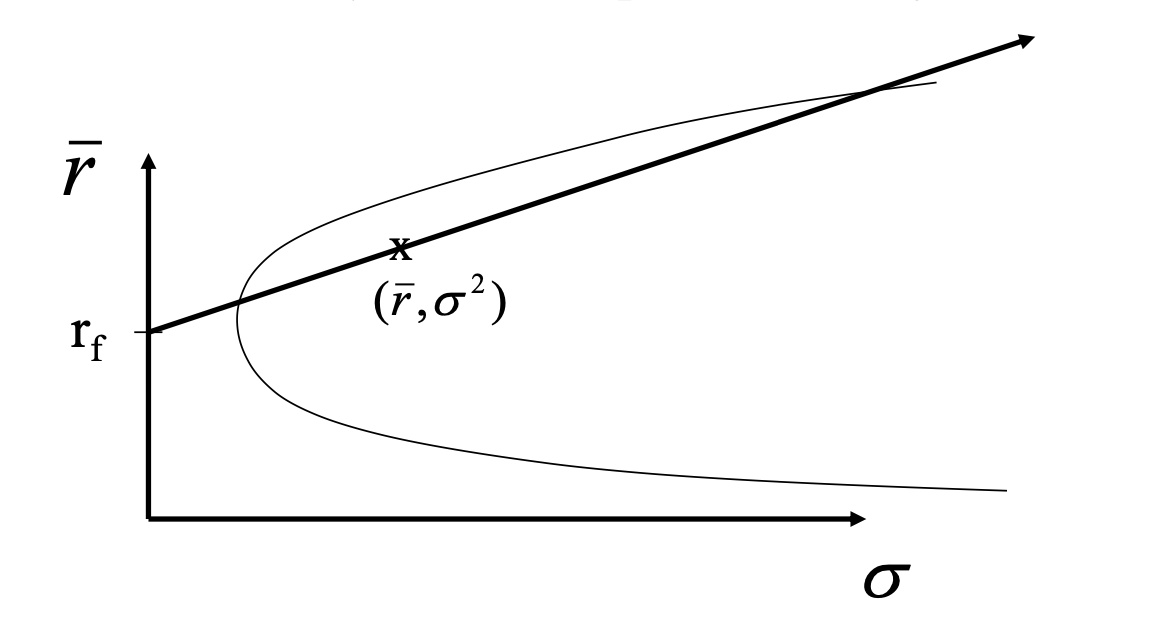
\includegraphics[scale=0.4]{riskfree.png} 
\end{center}

\subsubsection{One-Fund Theorem}
Assuming (i) short selling is allowed, (ii) all assets are risky, and (iii) all investors have the same estimates of mean, variance, and covariance,  there is a single fund $F$ of risky assets, such that any efficient portfolio can be constructed as a combination of the fund $F$ and the risk free asset.  \\ \\ The one-fund is the fund of risky assets that results in the maximum slope with the risk-free rate.  The slope is given by 
$$ slope =  \frac{ \bar{r}_{fund} - r_f}{\sigma_{fund}}$$
Getting the weights of the one fund theorem is just the following optimization problem:
\begin{align*}
(\bar{r}_k - r_f) - \lambda \left( \sum_{j=1}^n w_j \sigma_{kj} \right) &= 0  \\
 \sum_{j=1}^n \lambda w_j \sigma_{kj}  &= (\bar{r}_k - r_f) \\
 \sum_{j=1}^n v_j \sigma_{kj}  &= (\bar{r}_k - r_f)  \\
 w_j &= \frac{v_j}{\sum_{i=1}^n v_i}
\end{align*}

\pagebreak
\section{Capital Asset Pricing Model (CAPM)}
\subsection{Market Equilibrium}
A \textbf{market portfolio} is defined to be a portfolio of every stock in the market in proportion to the that stock's representation on the entire market.  Each assets weight in the market portfolio is 
$$ w_i = \frac{\$ \text{ value of asset } i}{\$ \text{ value of market}}$$
These weights are called \textbf{capitalization weights}.

\subsection{Pricing Model}
The Capital Asset Pricing Model makes the following assumptions:
\begin{enumerate}
\item All investors are Markowitz mean-variance investors
\item Short selling is allowed
\item There exists a risk-free asset 
\item Investors share the same predictions for means, variances, covariances, etc.
\end{enumerate}
The theorem states that if the market portfolio $M$ is efficient, the expected return $r_i$ of any asset $i$ satisfies 
$$ r_i - r_f = \beta_i (\bar{r}_m - r_f) \quad \quad \quad \beta_i = \frac{\sigma_{iM}}{\sigma^2_M}$$  
\\ 
\begin{center}
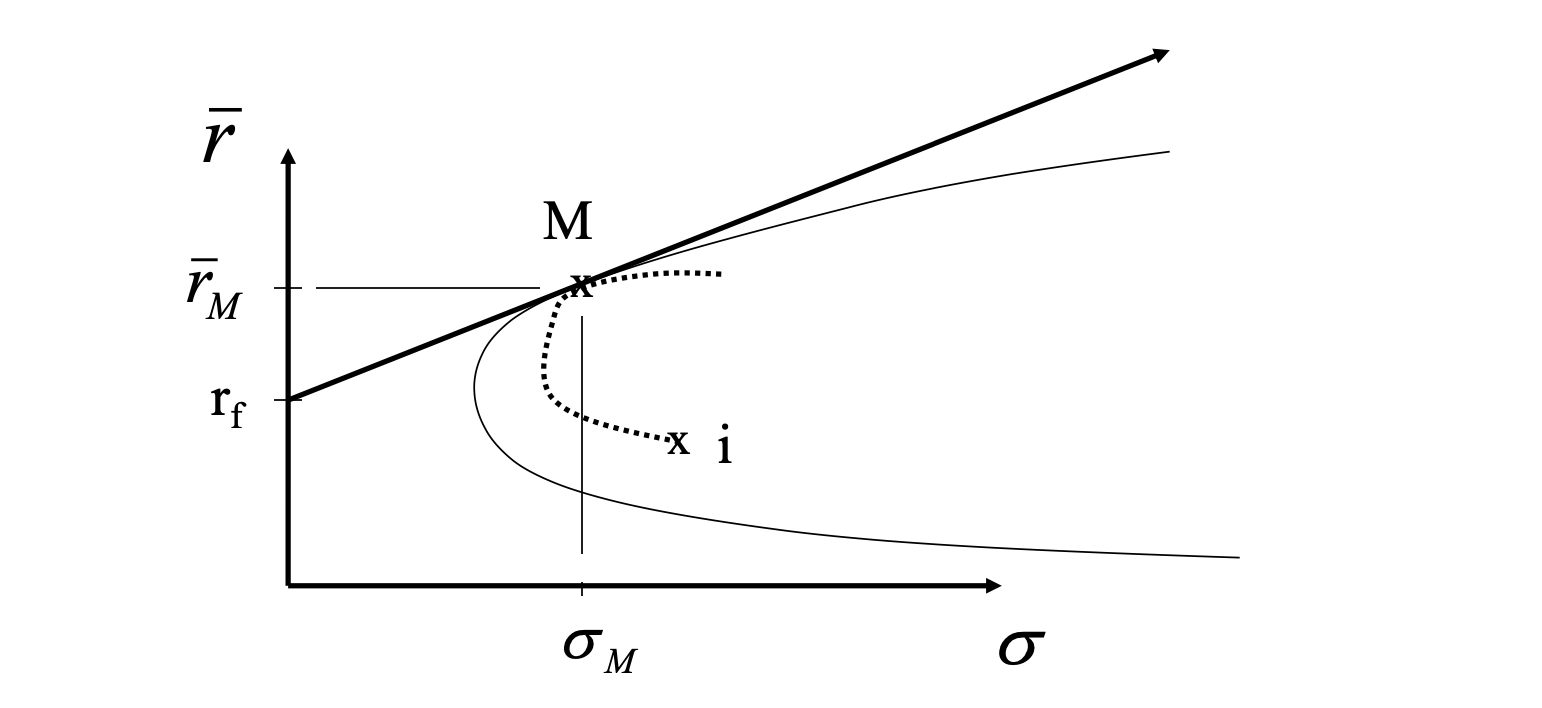
\includegraphics[scale=0.6]{capm.png} 
\end{center}

\subsection{Security Market Line}
\begin{itemize}
\item All CAPM securities lie along this line 
\begin{center}
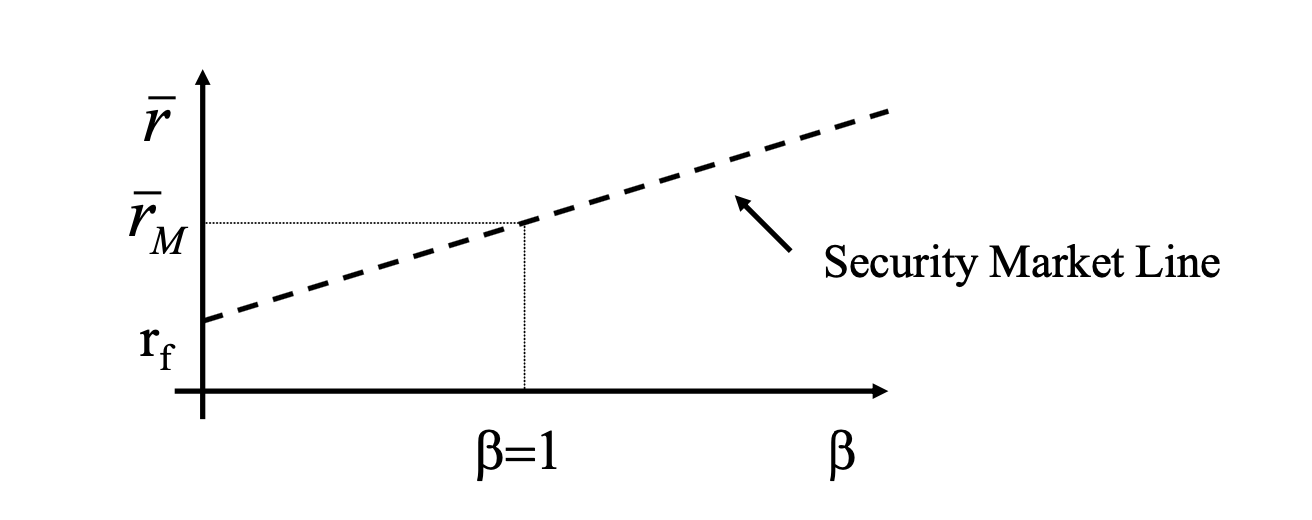
\includegraphics[scale=0.4]{sml.png} 
\end{center}
\item The correlation with market $\beta$ determines the expected return
\begin{itemize}
\item $\beta_i = 0 \rightarrow r_i = r_f + 0 \cdot (\bar{r}_m - r_f) = r_f $
\item $\beta_i = 1 \rightarrow r_i = r_f + 1 \cdot (\bar{r}_m - r_f) = \bar{r}_m $
\item $\beta_i = 2 \rightarrow r_i = r_f + 2 \cdot (\bar{r}_m - r_f) = 2\bar{r}_m -r_f $
\end{itemize}
\item $\beta$ also determines the movement with the market
\end{itemize}

\subsection{Risk}
The covariance of an asset, $r_i$ can be given as 
$$ \sigma_i^2 = COV(r_i, r_i) = \beta_i^2\sigma^2_M + var(\epsilon_i)$$
This risk is broken up into two components:
\begin{itemize}
\item $\beta_i^2\sigma^2_M \rightarrow $ systematic risk, associated with the market as a whole
\item $ var(\epsilon_i) \rightarrow $ non-systematic,  idiosyncratic, specific risk uncorrelated with market reduced by diversification
\end{itemize}
\begin{center}
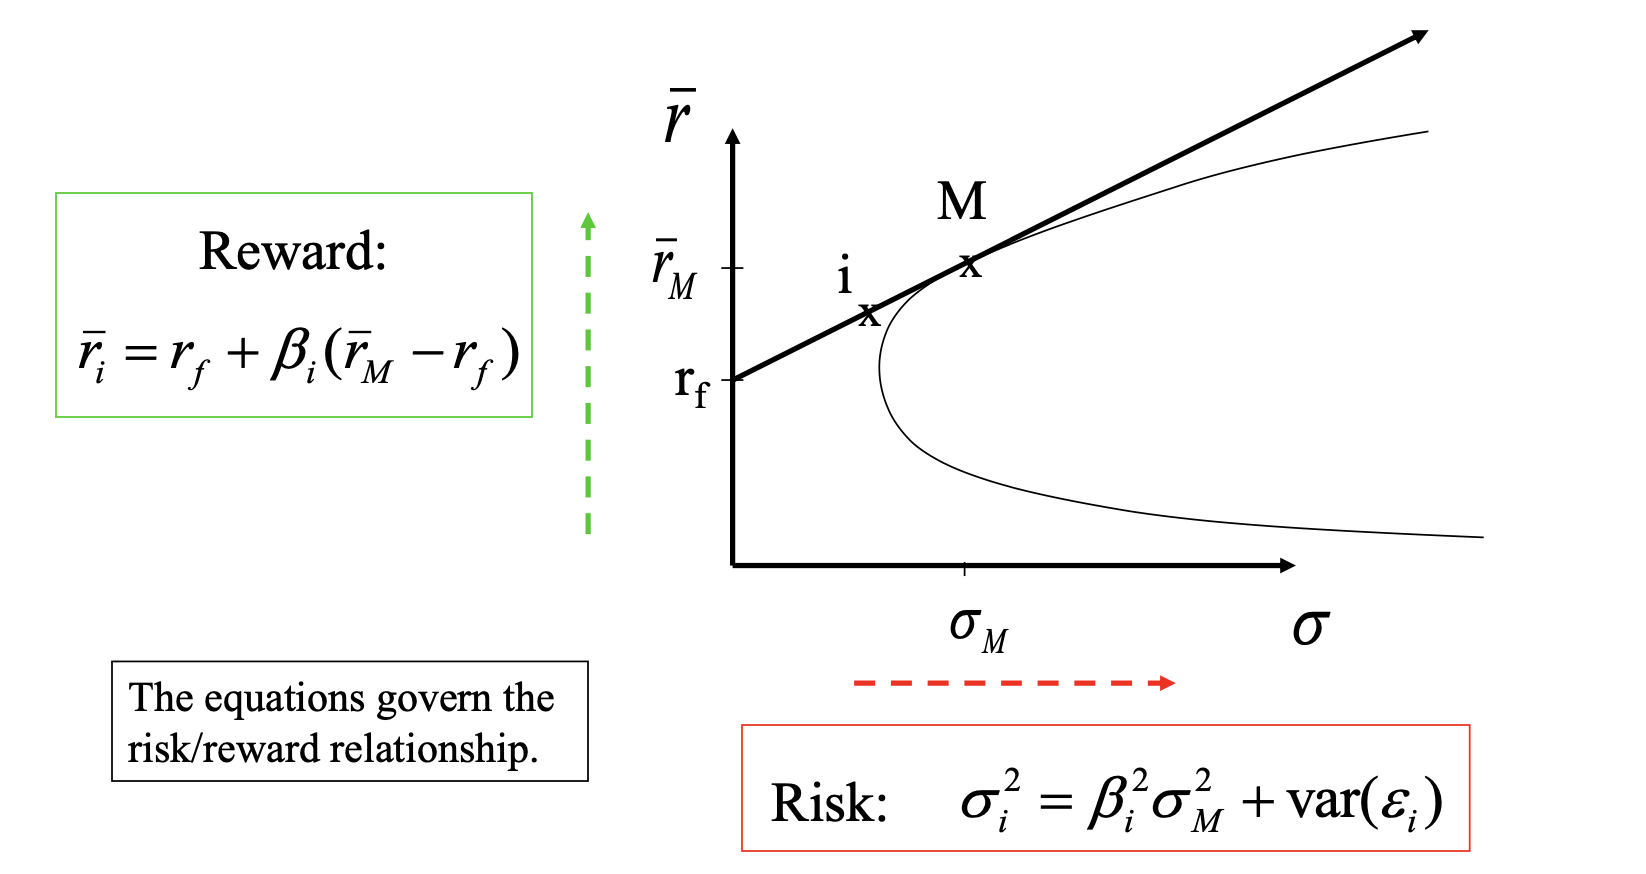
\includegraphics[scale=0.4]{rkrw.png} 
\end{center}

\subsection{Implications}
\begin{itemize}
\item According to our theory, the only portfolio of risky assets you should be holding is the market
\item Hence you are only rewarded the (expected return) for risk related to the market 
\item Risk is measured by $\beta$, not the variance of your asset
\item Return on an asset is determined by how it fits into the market portfolio, not by its characteristic alone.
\end{itemize}

\subsection{$\beta$ of a Portfolio}
Given a portfolio, $r_p = w_1r_1 + w_2r_2 + \cdots + w_nr_n$, the $\beta$ of the portfolio can be given as 
\begin{align*}
\beta_p &= \frac{COV(r_p, r_M}{VAR(r_M)} \\
&= \frac{COV(w_1r_1 + w_2r_2 + \cdots + w_nr_n, r_M)}{VAR(r_M)} \\
&=\frac{w_1COV(r_1, r_M) + w_2COV(r_2, r_M) + \cdots + w_nCOV(r_n, r_M)}{VAR(r_M)} \\
&= w_1\beta_1 + w_2\beta_2 + \cdots + w_n\beta_n
\end{align*}
\pagebreak

\section{Options}

\subsection{Financial Derivatives}
A financial derivative is a financial instrument whose value depends on the values of other more basic underlying financial instruments or variables \textit{(i.e. options)}
\subsection{Call Options}
A call option is a derivative that gives the owner the right but not obligation to buy a certain asset by a certain date (maturity) for a certain price (strike price). The seller of the call option must deliver the underlying asset at the strike price if owner decides to buy.  There are two main types of options: 
\begin{itemize}
\item \textbf{American:} Can be exercised at any time in its life
\item \textbf{European:} Can only be exercised at maturity (we only deal with this in MIE375) 
\end{itemize}
In general, option payoffs are determined by the price of the underlying asset at maturity
\begin{center}
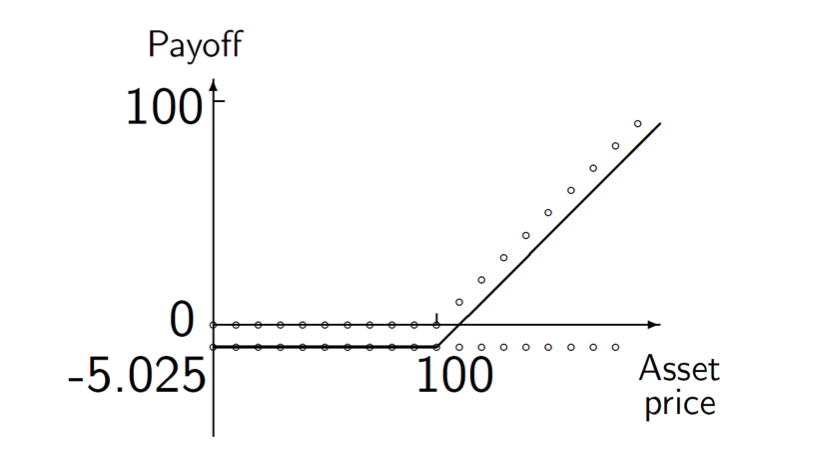
\includegraphics[scale=0.4]{call.png} 
\end{center}
\subsection{Put Options }
A put option gives the owner the right but not the obligation to sell a certain date (maturity) for a certain price (strike price). The seller of the put option must buy the underlying asset at the strike price if the owner decides to sell the asset. 
\begin{center}
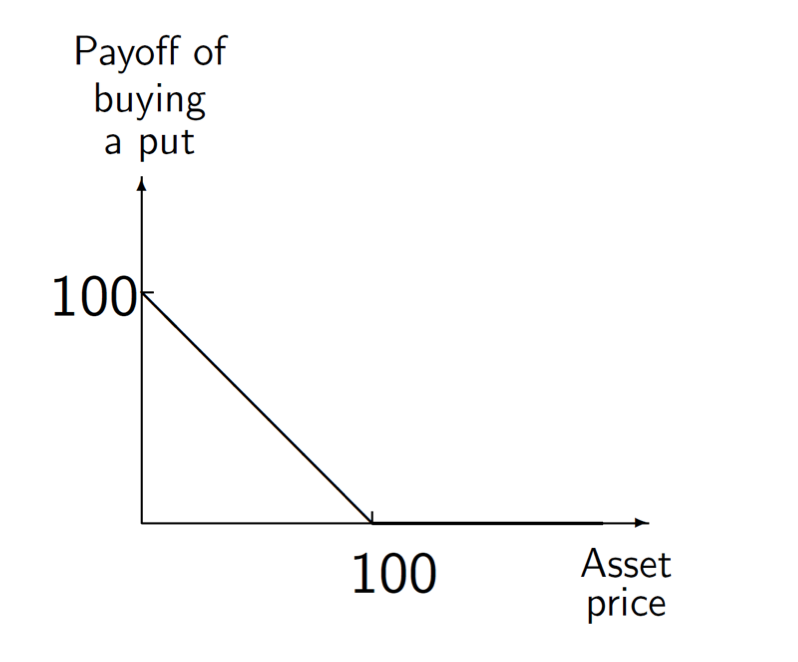
\includegraphics[scale=0.4]{put.png} 
\end{center}

\subsection{Exchange Traded vs Over-the-Counter}
Options are contracts that are financial instruments. They can be traded just like stocks on an exchange. Custom options can also be constructed over the counter.
\begin{itemize}
\item \textbf{Exchange Traded:} Mostly electronic trading; contracts are standardized in terms of strike prices and there is virtually no credit risk. 
\item \textbf{Over-the-Counter:} Contracts can be non-standard and there is a small amount of credit risk still 
\end{itemize}

\subsection{Types of Option Traders}
\begin{itemize}
\item \textbf{Hedgers:} Protect against adverse movements
\item \textbf{Speculators:} Take position on the direction of asset
\end{itemize}

\subsection{Option Portfolios}
Consider a portfolio of one call option and one put option on the same underlying asset with some maturity and strike price of $\$100 $. This strategy is called a \textbf{straddle} and has a positive value as long as the underlying asset price at maturity is not a 100. \\ \\ Another important application is construction portfolio overlays \textit{(e.g. covered call portfolios)}
\begin{itemize}
\item \textbf{Benefit:} Receive money from selling options (will improve portfolio returns)
\item\textbf{Risk:} Price of stocks may go up a lot in which case you have to deliver the stocks to the buyers of the call options at lower strike prices.
\end{itemize}

\subsection{Put-Call Parity}
$$ C + \frac{K}{(1+r)^T} = P +S $$ 
\begin{itemize}
\item $ C \rightarrow$ price of call option with strike price $k$
\item $ P \rightarrow$ price of put option with strike price $k$
\item $ S \rightarrow$ current price of one share
\item $ T \rightarrow$ maturity of call and put (same)
\item $ r \rightarrow$ interest rate
\end{itemize}

\pagebreak







\end{document}
